\documentclass[conference]{IEEEtran}
\usepackage[ngerman]{babel}
\usepackage[utf8]{inputenc}
\usepackage[T1]{fontenc}
\usepackage{graphicx}
\usepackage{caption}
\usepackage{subcaption}

\begin{document}
\title{Netzwerk-Service-Assurance-Tests über verteilte Systeme auf dem
TU Clausthal Campus}
\author{\IEEEauthorblockN{Christian Rebischke}
\IEEEauthorblockA{Technische Universität Clausthal\\
Rechenzentrum\\
Email: Christian.Rebischke@tu-clausthal.de}}

\maketitle

\begin{abstract}
Um eine gleichbleibende Netzqualität innerhalb des Netzes der
TU Clausthal zu gewährleisten, werden Computersysteme auf dem
Campus verteilt, um Service-Assurance-Tests durchzuführen. Diese
Tests sollen eine gleichbleibende und stabile Verbindung garantieren
und beim Abweichen von Messergebnissen einen Netzwerkadministrator
alarmieren. Die Ergebnisse sollen in einer Datenbank gespeichert und
für die weitere Verwertung gefiltert und optimiert
werden. Dabei ist geplant, die Masse an Computersystemen mit
State-of-the-Art-Orchestration und Config-Management-Tools im
Schwarm zu administrieren.
\end{abstract}

\IEEEpeerreviewmaketitle

\section*{Problemstellung}
Das Netz der TU Clausthal erstreckt sich über mehrere Standorte.
Teilweise liegen diese Standorte nicht in Clausthal selbst, wie
beispielsweise das EFZN in Goslar. Dementsprechend schwierig gestaltet
sich die Wartung und der Betrieb des Netzes. So kann auf Netzeinbrüche
etwa nur reaktiv nach Meldung des Problems reagiert werden. Es existiert
zwar ein Monitoring-System, welches die Verfügbarkeit von einzelnen
Diensten überprüft, jedoch erfolgt diese Messung nur von einem Punkt aus
und gibt nur binäre Statuswerte zurück (Dienst läuft oder Dienst läuft
nicht). Dementsprechend fehlen Informationen um die Verfügbarkeit von
Diensten und deren vollständige Funktion von mehreren Messpunkten aus zu
garantieren. Beispielsweise ist es möglich, dass ein Dienst zwar vom
zentralen Monitoring-Server aus erreichbar ist, aber aus einem einzelnen
Institut der Zugriff auf den Dienst nur eingeschränkt oder sogar gar
nicht möglich ist. Besonders Dienste wie \textit{Domain Name System}
(DNS) sind auf schnelle Verbindungen angewiesen. Eine zu hohe Latenz
zwischen einem Client und dem Dienst führt unweigerlich zu für den
Nutzer sichtbaren Konsequenzen (Zum Beispiel verzögerte Seitenaufrufe beim
Web-Browsing).
\section*{Lösungsansatz}
Als ersten Lösungsansatz ist ein System aus mehreren verteilten
Computern geplant. Die einzelnen Computer dienen als Messpunkte. Von den
einzelnen Messpunkten können dann Latenz- und Delay-Tests durchgeführt
werden. Die von den Messpunkten gesammelten Daten werden dann zur
weiteren Auswertung und grafischen Aufbereitung an ein System bestehend
aus einer Datenbank und einem Webserver gesendet. Die Latenz- und
Delay-Tests werden mit einer gängigen Programmiersprache implementiert.
Zur einfachen Verwaltung der verteilten Computern wird ein modernes
Config-Management-System benutzt.
\begin{figure}[h]
    \centering
    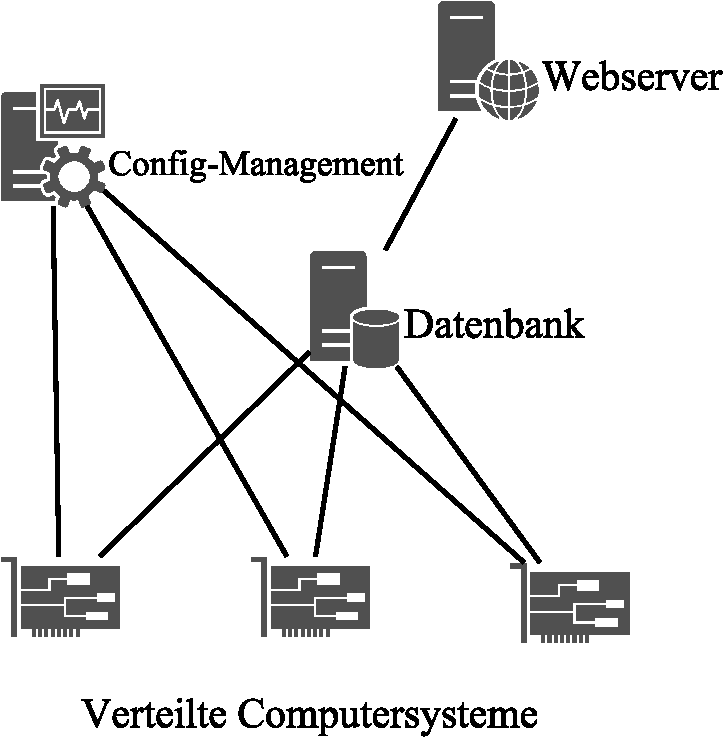
\includegraphics[width=0.5\textwidth]{figures/network.pdf}
    \caption{Netzwerk-Grundriss des Projekts}\label{fig:1}
\end{figure}

\section*{Danksagung}
Ich danke dem Rechenzentrum der TU Clausthal, dass ich dort meine
Bachelor-Arbeit schreiben darf.
\end{document}
